\chapter{Results}

\section{Scalability of the training time of the ML models} % High-performance computing (HPC) results}

Since the BGS dataset contains about 800000 data points, the training of algorithms, model selection, and validation can be too demanding, in processing and memory. Therefore, it is necessary to evaluate how the training time scales with the data when running in the High-Performance Computing (HPC) cluster of the University, taking account several variables as the number of processors to run in parallel the algorithm and the resources requested to the cluster. In particular, we will focus on the following variables:
\begin{align*}
m &= \text{Requested memory to solve the job [Gb]},\\
n_{jobs} &= \text{Number of jobs to run in parallel},\\
ppn &= \text{Requested processors per node},\\
n &= \text{size of the dataset used},\\
M &= \frac{n_{jobs} \times n}{ppn \times m}.
\end{align*}
\begin{figure}[ht!]
	\centering
	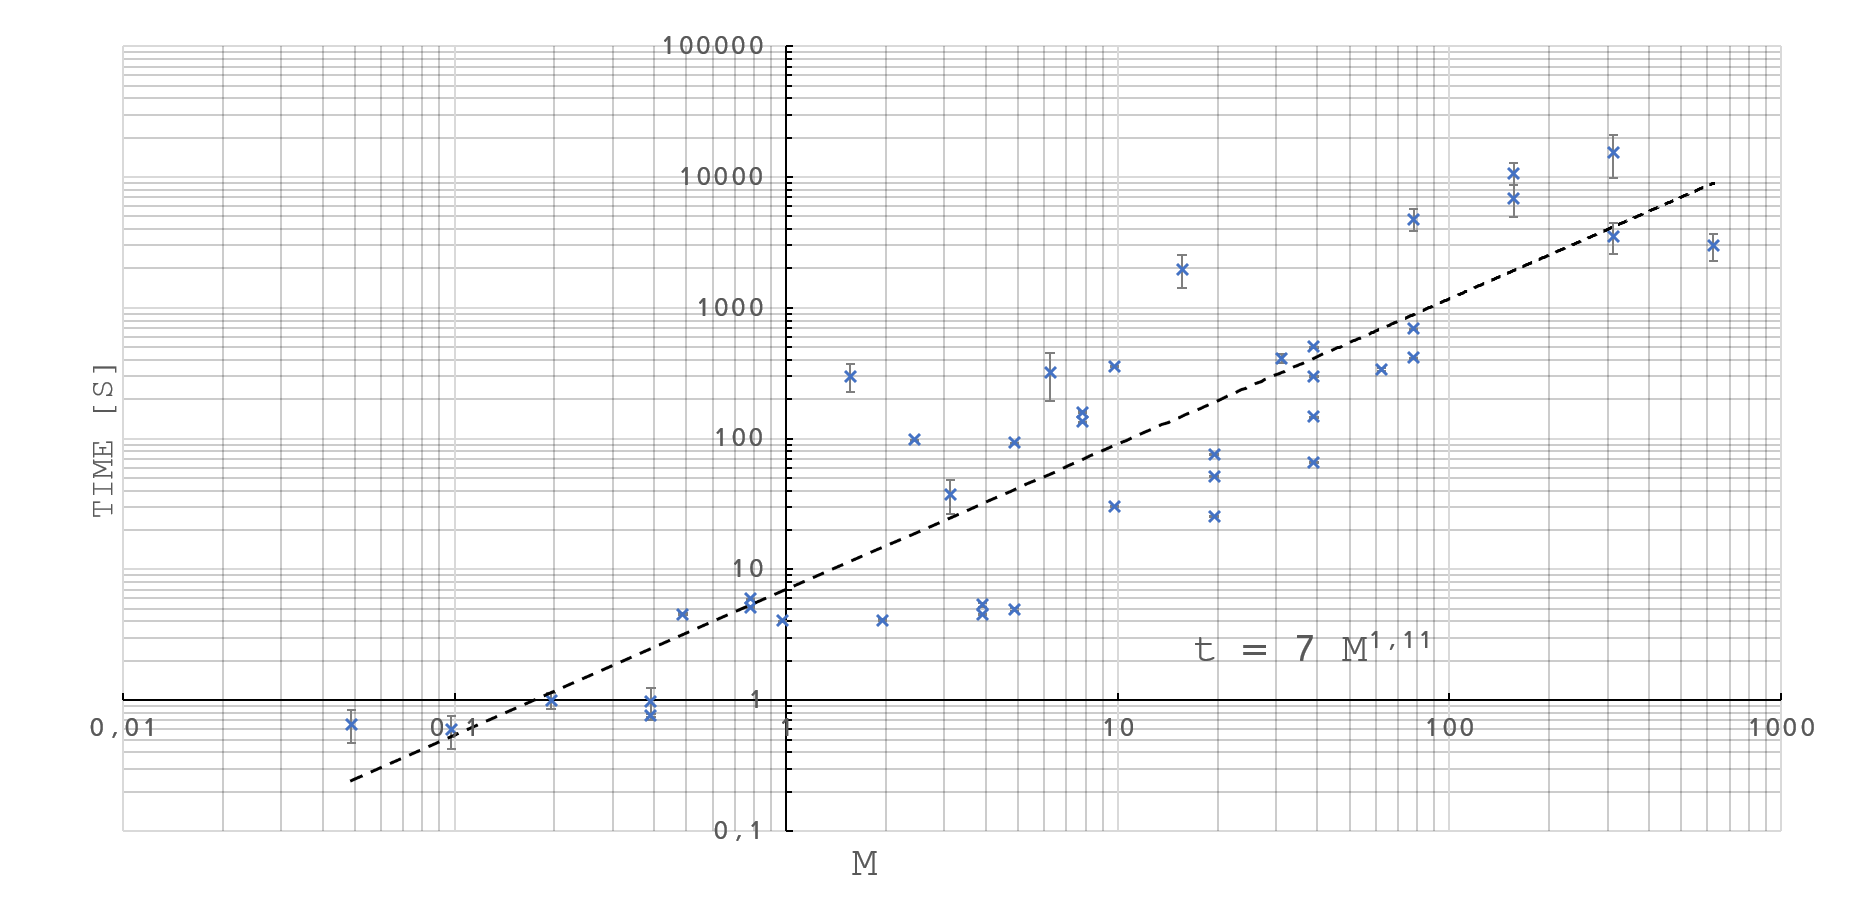
\includegraphics[width=1.0\linewidth]{TeX_files/Imagenes/hpc_results}
	\caption{Time as a function of requested memory, number of data points and jobs used to train the model.}
	\label{fig:hpcresults}
\end{figure}

The variable $M$ measures the relationship between the requested resources and the resources used. Figure \ref{fig:hpcresults} shows how time increases as a function of variable M. Note that $M^{-1}$ can be seen as a 'unitary memory', that is, the memory used per data per processor,
\begin{equation*}
M^{-1} = \frac{m}{p_u \times n},
\end{equation*}
where $p_u = n_{jobs}/ppn$ is the fraction of the requested processors that is actually being used by the parallel code. Therefore, when $M$ is big, it means that there is too much data per memory per processor, and the time to train the model is too high. It is worth mentioning that the time was measured for the kernel ridge regression model particularly, using grid search and 3-fold cross-validation. Others model may be faster or slower to train, but the behavior should be the same. From Figure \ref{fig:hpcresults} we see that the time of training for a given $M$ can be approximated by the relation
\begin{equation}
t = 7M^{1.11} [s].
\end{equation}

This results have to be constrained to the waiting time in queue of the cluster, in general, the smaller M, the best time, but that means, using small dataset or increasing the resources, but for the second option, the more resources you request, the longer the queue and waiting time to execute the code. It was found that a configuration with \textbf{$n_{jobs} = 16$, $ppn = 32$, $m = 128 Gb$ and $n = 100000$}, gives good results. n is critical since it determines how well the model will learn, 100000 data points work very well as it will be shown in the next sections.  

\section{Model results}

We train and test three models, namely a KRR, an SVR, and an ensemble model. We divided the original BGS dataset into a 75 - 25 train-test set, from the 75 \%, each model was trained on a subset of size 100.000, as mentioned in the previous section. To account for the bias, we trained the same model in tree 100.000 subsets and the results were averaged. The selection of the model hyperparameters was made by using grid search a 3-fold cross-validation, using an 80-20 development-evaluation scheme. 

\subsection{Support Vector Regression (SVR) Model}

The grid-search and cross-validation on the train-development set use the $r^2$ measure to select the best parameters. 

\begin{verbatim}
--------------------------------------------------------------------------
Model 1:
Best parameters set found on development set:

{'gamma': 0.1, 'C': 1, 'kernel': 'rbf'}

Grid scores on development set:

0.877 (+/-0.001) for {'gamma': 0.001, 'C': 1, 'kernel': 'rbf'}
0.927 (+/-0.011) for {'gamma': 0.1, 'C': 1, 'kernel': 'rbf'}
0.848 (+/-0.017) for {'gamma': 1, 'C': 1, 'kernel': 'rbf'}
0.896 (+/-0.001) for {'gamma': 0.001, 'C': 10, 'kernel': 'rbf'}
0.924 (+/-0.010) for {'gamma': 0.1, 'C': 10, 'kernel': 'rbf'}
0.870 (+/-0.013) for {'gamma': 1, 'C': 10, 'kernel': 'rbf'}
0.898 (+/-0.006) for {'gamma': 0.001, 'C': 100, 'kernel': 'rbf'}
0.922 (+/-0.007) for {'gamma': 0.1, 'C': 100, 'kernel': 'rbf'}
0.868 (+/-0.020) for {'gamma': 1, 'C': 100, 'kernel': 'rbf'}

r2 score computed on the full evaluation set:

0.928

--------------------------------------------------------------------------
Model 2:

Best parameters set found on development set:

{'gamma': 0.1, 'C': 1, 'kernel': 'rbf'}

Grid scores on development set:

0.878 (+/-0.002) for {'gamma': 0.001, 'C': 1, 'kernel': 'rbf'}
0.928 (+/-0.007) for {'gamma': 0.1, 'C': 1, 'kernel': 'rbf'}
0.859 (+/-0.020) for {'gamma': 1, 'C': 1, 'kernel': 'rbf'}
0.892 (+/-0.002) for {'gamma': 0.001, 'C': 10, 'kernel': 'rbf'}
0.919 (+/-0.019) for {'gamma': 0.1, 'C': 10, 'kernel': 'rbf'}
0.859 (+/-0.010) for {'gamma': 1, 'C': 10, 'kernel': 'rbf'}
0.902 (+/-0.003) for {'gamma': 0.001, 'C': 100, 'kernel': 'rbf'}
0.909 (+/-0.006) for {'gamma': 0.1, 'C': 100, 'kernel': 'rbf'}
0.861 (+/-0.020) for {'gamma': 1, 'C': 100, 'kernel': 'rbf'}

r2 score computed on the full evaluation set:

0.92
--------------------------------------------------------------------------
Model 3:

Best parameters set found on the development set:

{'gamma': 0.1, 'C': 1, 'kernel': 'rbf'}

Grid scores on development set:

0.879 (+/-0.003) for {'gamma': 0.001, 'C': 1, 'kernel': 'rbf'}
0.926 (+/-0.019) for {'gamma': 0.1, 'C': 1, 'kernel': 'rbf'}
0.847 (+/-0.008) for {'gamma': 1, 'C': 1, 'kernel': 'rbf'}
0.898 (+/-0.005) for {'gamma': 0.001, 'C': 10, 'kernel': 'rbf'}
0.921 (+/-0.015) for {'gamma': 0.1, 'C': 10, 'kernel': 'rbf'}
0.868 (+/-0.009) for {'gamma': 1, 'C': 10, 'kernel': 'rbf'}
0.901 (+/-0.005) for {'gamma': 0.001, 'C': 100, 'kernel': 'rbf'}
0.891 (+/-0.018) for {'gamma': 0.1, 'C': 100, 'kernel': 'rbf'}
0.853 (+/-0.012) for {'gamma': 1, 'C': 100, 'kernel': 'rbf'}

r2 score computed on the full evaluation set:

0.93

\end{verbatim}
\begin{figure}[th!]
	\centering
	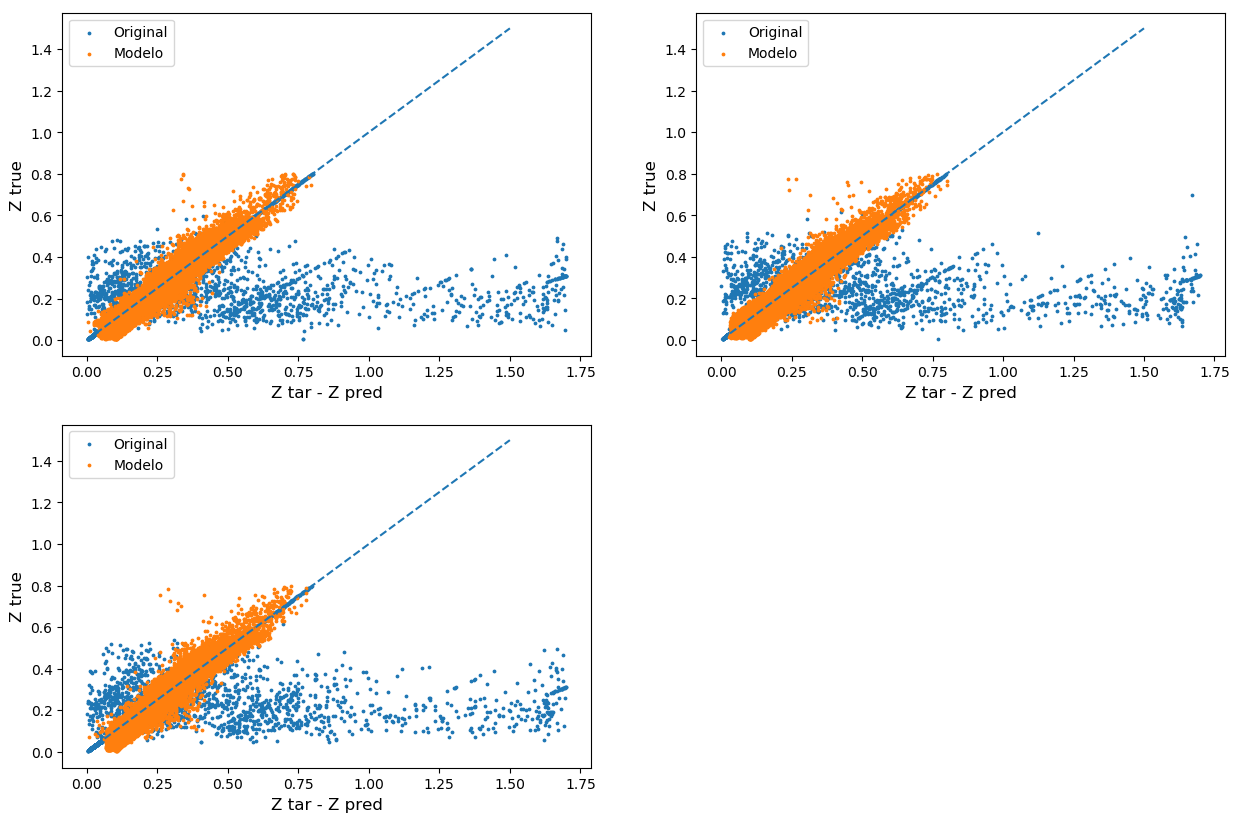
\includegraphics[width=1.0\linewidth]{TeX_files/Imagenes/svr-train}
	\caption{Results on the training set after training the SVR model.}
	\label{fig:svr-train}
\end{figure}
The results on the training set of the best models are shown in Figure \ref{fig:svr-train}. On training, the model shows good results by gathering the blue dots (original data)over the orange dots (the model results after applying it to the training data). The blue scatter is substantially diminished and the data is clustered along de TRUEZ = TARZ line, However, the data is not entirely over the line, but in a wide range. Figure \ref{fig:svr-test} shows the result on the evaluation set for each model. 
\begin{figure}[th!]
	\centering
	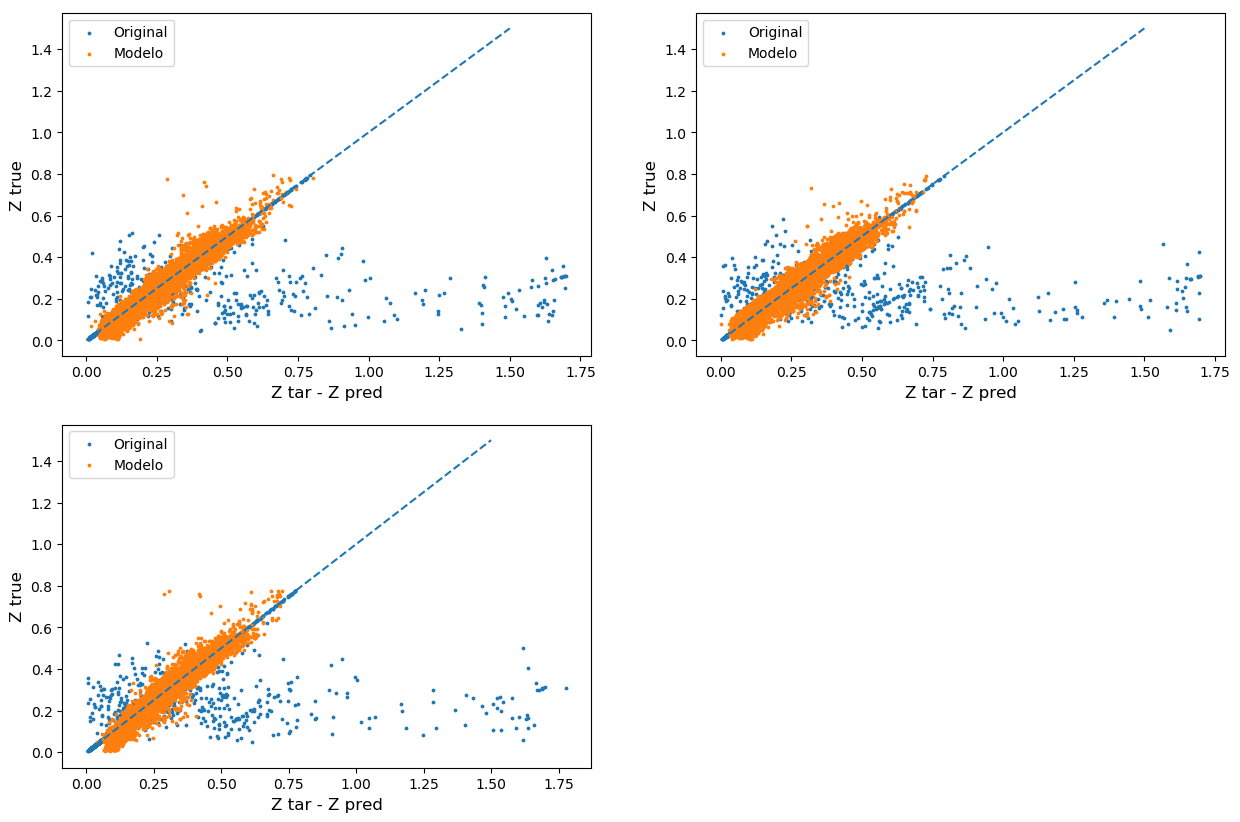
\includegraphics[width=1.0\linewidth]{TeX_files/Imagenes/svr-test}
	\caption{Results of each model on the development set.}
	\label{fig:svr-test}
\end{figure}
Figure \ref{fig:svr-test} shows how the model generalize to unseen data. The gathering capacity of the model to move the blue dots towards the TRUEZ = TARZ line present on the training set is also visible on the evaluation set, were the $r^2$ scores reaches 93\% only. 
\subsection{Kernel Ridge Regression (KRR) Model}

The grid-search and cross-validation on the train-development set use the $r^2$ measure to select the best parameters. 

\begin{verbatim}
--------------------------------------------------------------------------
Model 1:
Best parameters set found on development set:

{'alpha': 0.0001, 'gamma': 0.2, 'kernel': 'rbf'}

Grid scores on development set for r2:

0.986 (+/-0.002) for {'alpha': 0.001, 'gamma': 0.1, 'kernel': 'rbf'}
0.988 (+/-0.002) for {'alpha': 0.001, 'gamma': 0.2, 'kernel': 'rbf'}
0.987 (+/-0.002) for {'alpha': 0.0001, 'gamma': 0.1, 'kernel': 'rbf'}
0.989 (+/-0.002) for {'alpha': 0.0001, 'gamma': 0.2, 'kernel': 'rbf'}

r2 score computed on the full evaluation set:

0.990
--------------------------------------------------------------------------
Model 2:
Best parameters set found on the development set:

{'alpha': 0.001, 'gamma': 0.2, 'kernel': 'rbf'}

Grid scores on development set for r2:

0.986 (+/-0.001) for {'alpha': 0.001, 'gamma': 0.1, 'kernel': 'rbf'}
0.988 (+/-0.002) for {'alpha': 0.001, 'gamma': 0.2, 'kernel': 'rbf'}
0.987 (+/-0.002) for {'alpha': 0.0001, 'gamma': 0.1, 'kernel': 'rbf'}
0.987 (+/-0.004) for {'alpha': 0.0001, 'gamma': 0.2, 'kernel': 'rbf'}

r2 score computed on the full evaluation set:

0.988
--------------------------------------------------------------------------
Model 3:
Best parameters set found on the development set:

{'alpha': 0.001, 'gamma': 0.2, 'kernel': 'rbf'}

Grid scores on development set r2:

0.987 (+/-0.001) for {'alpha': 0.001, 'gamma': 0.1, 'kernel': 'rbf'}
0.988 (+/-0.002) for {'alpha': 0.001, 'gamma': 0.2, 'kernel': 'rbf'}
0.987 (+/-0.003) for {'alpha': 0.0001, 'gamma': 0.1, 'kernel': 'rbf'}
0.987 (+/-0.003) for {'alpha': 0.0001, 'gamma': 0.2, 'kernel': 'rbf'}

r2 score computed on the full evaluation set:

0.9899

\end{verbatim}
\begin{figure}[th!]
	\centering
	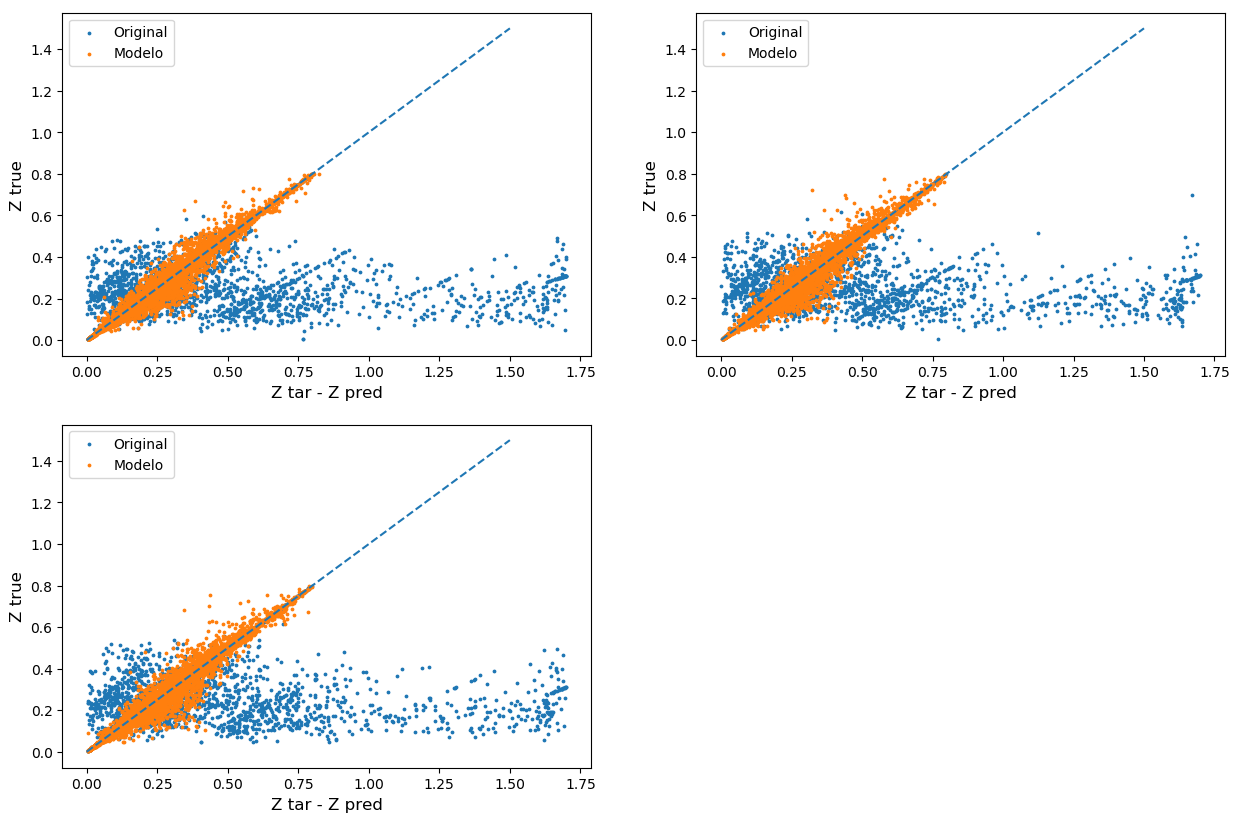
\includegraphics[width=1.0\linewidth]{TeX_files/Imagenes/krr-train}
	\caption{Results on the training set after training the KRR model.}
	\label{fig:krr-train}
\end{figure}
The results on the training set of the best models are shown in Figure \ref{fig:krr-train}. On training, the model shows better results than SVR by gathering the blue dots (original data)over the orange dots (the model results after applying it to the training data) on a tighter region. The blue scatter is substantially diminished and the data is clustered along de TRUEZ = TARZ line. Figure \ref{fig:krr-test} shows the result on the evaluation set for each model. 
\begin{figure}[th!]
	\centering
	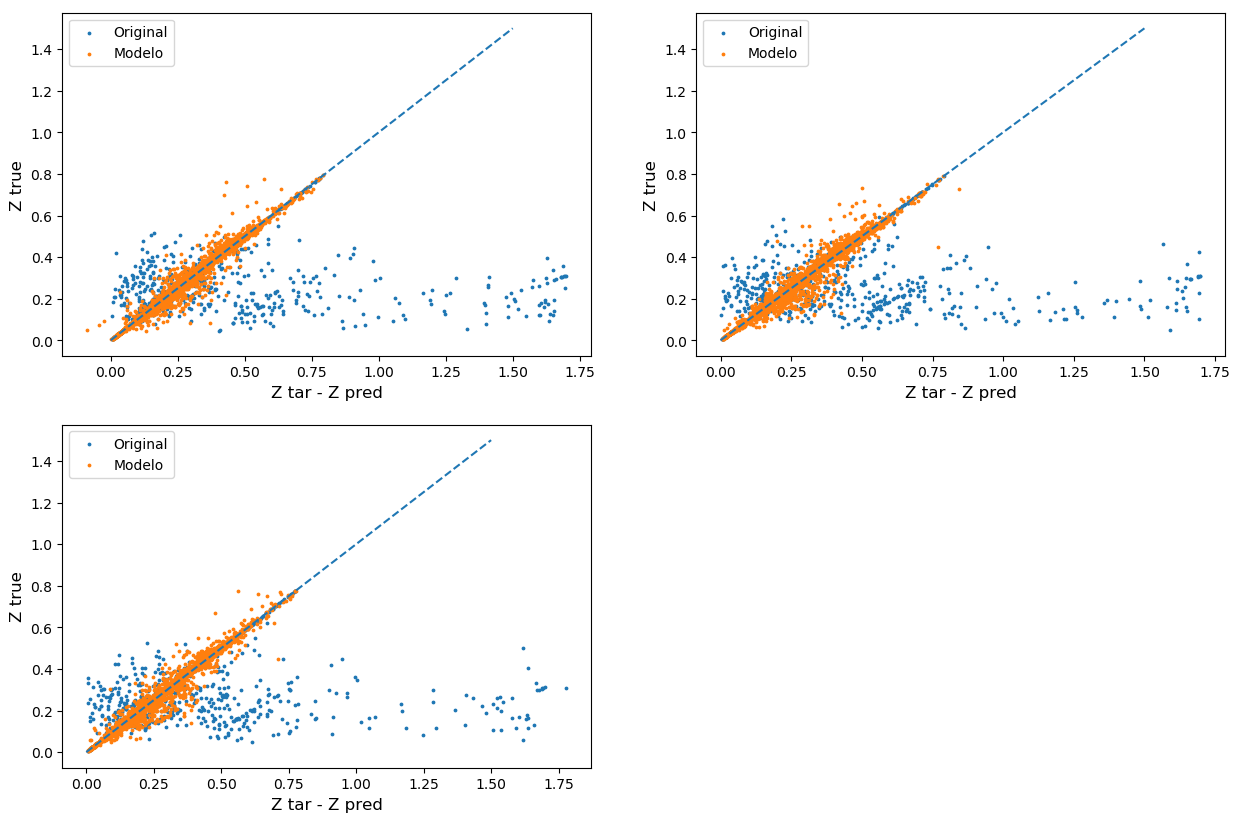
\includegraphics[width=1.0\linewidth]{TeX_files/Imagenes/krr-test}
	\caption{Results of each model on the development set.}
	\label{fig:krr-test}
\end{figure}
Figure \ref{fig:krr-test} shows how the model generalize to unseen data. The gathering capacity of the model to move the blue dots towards the TRUEZ = TARZ line present on the training set is also visible on the evaluation set, were the $r^2$ scores reaches 99\%, a more better result than that obtaining using SVR. 

\subsection{Model Ensemble}

The results from the KRR are much better than those of the SVR, also note that the KRR model takes about half the time to train. Given that we have three different models to predict on the same dataset, we have to make this model to predict a single output. For this, we try taking the maximum, the average or a weighted average of the model. 
\begin{figure}[h!]
	\centering
	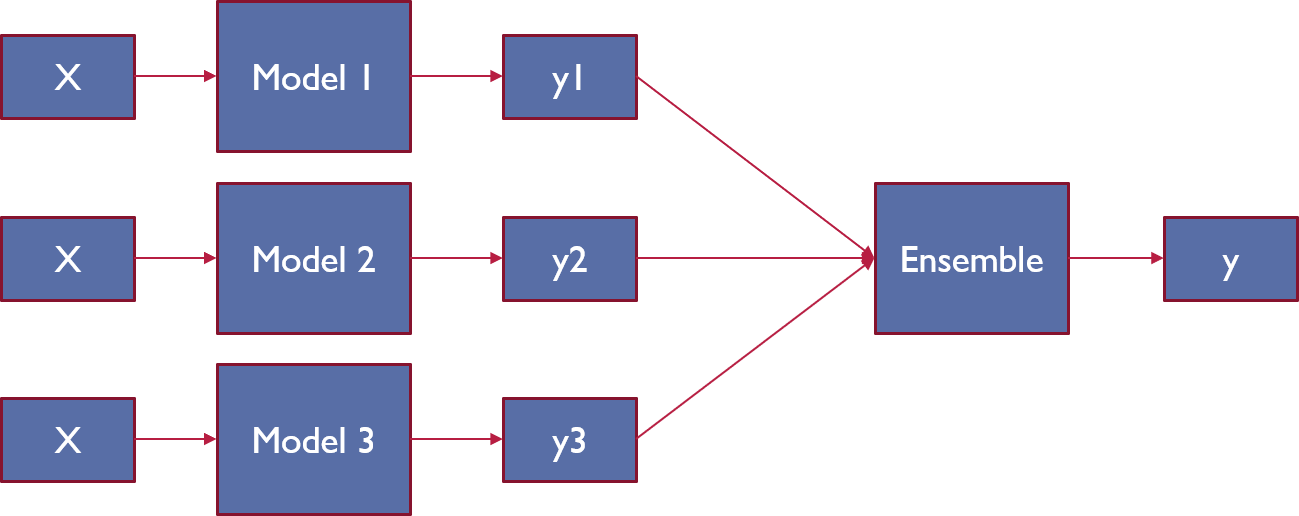
\includegraphics[width=1\linewidth]{TeX_files/Imagenes/ensemble_model}
	\caption{Graphic description of the ensemble model. It is formed based on the trained KRR models 1, 2 and 3.}
	\label{fig:ensemblemodel}
\end{figure}

Figure \ref{fig:ensemblemodel} shows this in a diagram, it is important to note that the ensemble is made over the \textbf{trained} models, that means that the parameters of the models are not re-learned in the ensemble. The only ensemble model that involves training, is the weighted average, where the weights are selected by training a linear model. The results of the models on the \textbf{test} subset (unseen 25\%) are shown in Table \ref{table:test-result}. 

\begin{table}[h!]
	\centering
	\begin{tabular}{|c|c|}
		\hline 
		Model & $r^2$ \\ 
		\hline 
		Model 1 & 0.958 \\ 
		\hline 
		Model 2 & 0.956 \\ 
		\hline 
		Model 3 & 0.962 \\ 
		\hline 
		Model avg & 0.962 \\ 
		\hline 
		Model max & 0.949 \\ 
		\hline 
		Model w & 0.983 \\ 
		\hline 
	\end{tabular} 
	\caption{Results on the \textbf{test} set}
	\label{table:test-result}
\end{table}

Table \ref{table:test-result} shows that the weighted average of the three models is the best model in terms of accuracy, taking into account that these are the predictions of the models on the totally-unseen test data corresponding to the 25\% of the original BGS dataset. 
\section{Model Selection}

The class of models evaluated is that of kernels models, the complexity of both, the SVR and the KRR is very similar, however, the KRR gave better results. This could be attributed to the lack of tuning of the $\epsilon$ parameter in SVR, due to the time of computation of SVR training. Smaller values of $\epsilon$ may result in a tighter region over the TRUEZ = TARZ line, therefore increasing the $r^2$. The weighted average model has at least 3 times more parameters that any model individually, its results are much better. Therefore, the best model that keeps simplicity and very good results is the weighted average model. 

\section{Conclusions}

We evaluated two types of kernels method, the support vector regression (SVR) and the kernel ridge regression (KRR). The dataset was split in a training part (75\%) and a test part (25\%). We trained each model three times on subsets of the training part of size 100.000, this subset was also subdivided in an 80-20 development - evaluation datasets for the application of grid search and cross-validation. The KRR gave better results than the SVR, also, the three KRR models were ensemble as a weighted average, where the weights were found using a linear regressor. The ensemble average KRR model reached an $r^2$ of 0.98 on the test set. 